\documentclass[10pt,a4paper]{article}
\usepackage[utf8]{inputenc}
\usepackage[italian]{babel}
\usepackage{amsmath}
\usepackage{amsfonts}
\usepackage{amssymb}
\usepackage{graphicx}
\usepackage{fullpage}
\usepackage{hyperref}
\usepackage{graphicx}
\usepackage{caption}
\usepackage{subcaption}

\author{Michele Carignani, Alessandro Lenzi}
\title{Analisi aggregata per ore}
\begin{document}

\maketitle

\section{Generazione dei grafi orari}

Per prima cosa i dati sono stati aggregati per ora. I dati originali del dataset 
%todo sistemare dataset
\href{https://dandelion.eu/datagem/telecom-mi-to-mi/description/}{Telecommunications - MI to MI} sono nel formato:
\begin{verbatim}
timestamp \t SourceId \t DestId \t Stregth
\end{verbatim}
e sono stati suddivisi in 24 file (uno per ogni ora) e aggregati, per cui
ogni file contiene (al massimo\footnote{poichè certi nodi possono non avere chiamate in uscita
in una certa fascia oraria.}) un record per ogni nodo nel formato:
\begin{verbatim}
SourceId \t DestId:Strength [\t DestId:Strength]
\end{verbatim}

A questo punto i pesi sugli archi (sopra chiamati \verb!Strength!) sono stati riscalati rispetto alla somma
dei valori della stella uscente di un nodo, ottenendo la probabilità di transire dal nodo $i$ al 
nodo $j$, ovvero:
$$ sumStrength_i = \sum_{j \in FS(i)} Strength_{ij} $$
$$ probability_{ij} = \frac{Strength_{ij}}{sumStrength_i} $$

\section{Ricerca delle componenti fortemente connesse}

Per ricercare le componenti fortemente connesse (in seguito CFC) è stato utilizzato l'algoritmo Tarjan
su un sotto insieme degli archi ''tagliati'' secondo il peso percentuale.

\subsection{Tagli}
Un taglio degli archi su un valore $x$ significa utilizzare per la visita solo gli archi con peso (ovvero valore di probabilità) maggiore o uguale a $x$. 
L'algoritmo esegue sampling sugli archi ($10^6$ sample) e calcola la distribuzione delle probabilità nella fascia oraria in esame. Su questa distribuzione calcola i percentili. L'algoritmo è stato eseguito con diversi tagli ai percentili 99, 95, 90 e 80.

\subsection{Strategie di visita}
\textbf{Le strategie di visita} utilizzate sono 5 e impiegano i dati del dataset 
\href{https://dandelion.eu/datagem/telecom-sms-call-internet-mi/description/}{"Telecommunications - SMS, Call, Internet - MI"}:
a partire dai record del formato
\begin{verbatim}
SquareID \t Timestamp \t .. ChiamateInUscita ..
\end{verbatim}
per ogni ora sono stati generati file con record
\begin{verbatim}
SquareID \t AggregatedCalls
\end{verbatim}
che permettono di capire quale sia il valore assoluto proporzionale a tutte le chiamate in uscita dallo square
$ID$ in una certa fascia oraria.
In questo modo è possibile iniziare la visita del grafo non da nodi ordinati lessicograficamente ma in ordine
(crescente o decrescente) di traffico in uscita.
Le strategie inoltre si differenziano per il modo di ordinare la stella uscente da un nodo.
Sono state provate diverse strategie:

\begin{itemize}
\item SCC1: visita il grafo in ordine crescente di traffico uscente,
selezionando prima gli archi con probabilità maggiore;
\item SCC2: visita i nodi per traffico decrescente e con archi selezionati per probabilità crescente;
\item SCC3: visita i nodi per traffico decrescente e gli archi per probabilità crescente;
\item SCC4: visita dei nodi per traffico crescente e archi per probabilità decrescente;
\item Stable: Esegue la ricerca delle componenti fortemente connesse selezionando i nodi in ordine crescente di traffico telefonico \textbf{giornaliero} uscente e gli archi in ordine di probabilità decrescente.
\end{itemize}
 
\section{Risultati}

\subsection{Statistiche}

In fig. \ref{img:probs} sono mostrate le statistiche sui pesi degli archi come probabilità sulle diverse
fasce orarie della giornata del 15 novembre.
\begin{figure}
 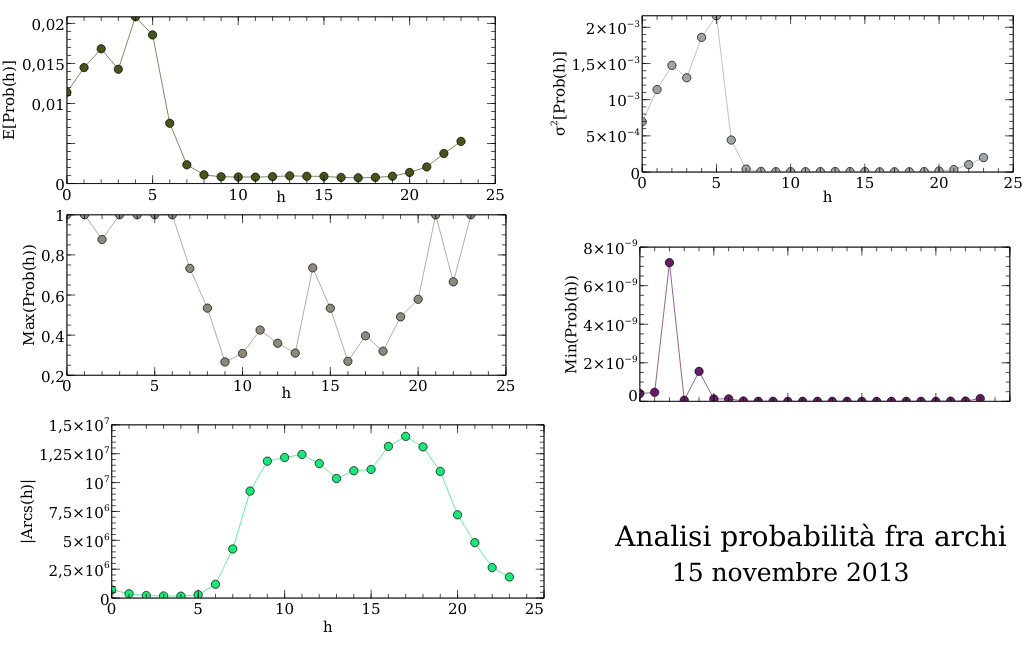
\includegraphics[scale=.6]{img/probs15nov.png}
 \caption{Statistiche sui pesi degli archi, 15 novembre. Sulle ascisse le fascie orarie, sulle ordinate le probabilità.}
 \label{img:probs}
\end{figure}

\subsection{Componenti Fortemente Connesse}

Le CFC sono state disegnate su mappe (utilizzando \verb!gnuplot!) assegnando una funzione $z$ alle celle di
coordinate $(x,y)$ così definita:
$$
z(x,y) =
\begin{cases}
0, & \text{se $(x,y)$ non appartiene ad alcuna CFC,} \\
10k, & \text{se $(x,y)$ appartiene alla k-esima CFC trovata.}
\end{cases}
$$

Perciò i seguenti grafici disegnagno le CFC nella loro posizione sulla Milano Grid.

\subsubsection{SCC1, taglio 0.005}
\label{scc1_0-005}
\begin{figure}
\centering

\begin{subfigure}[b]{1\textwidth}
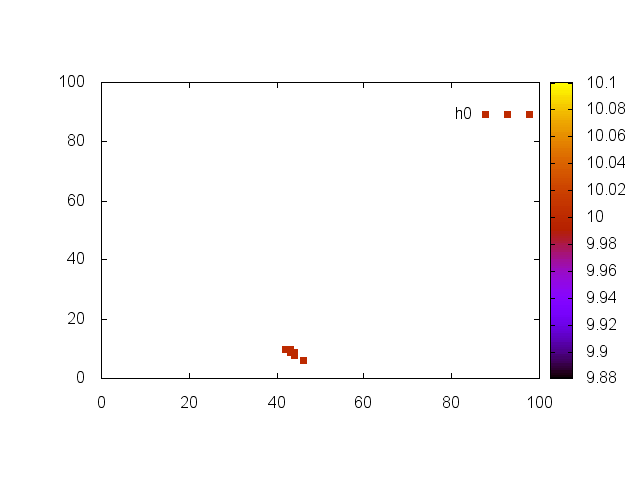
\includegraphics[scale=.3]{./img/stampe/scc1/0.png}
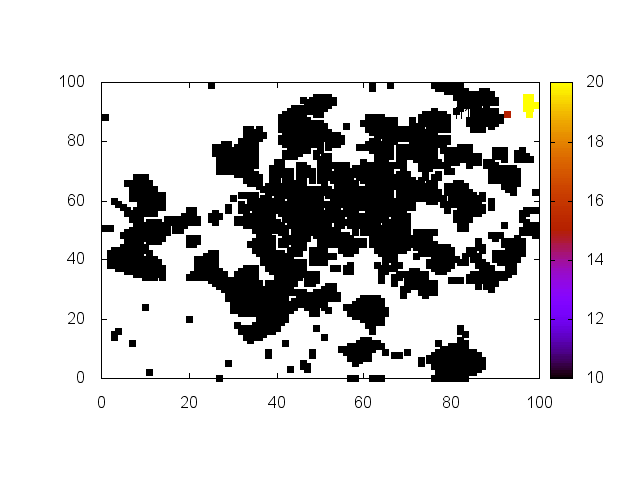
\includegraphics[scale=.3]{./img/stampe/scc1/1.png}
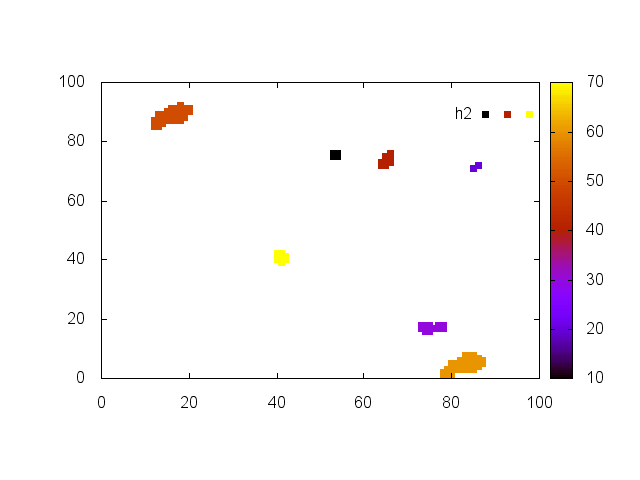
\includegraphics[scale=.3]{./img/stampe/scc1/2.png}
\end{subfigure}

\begin{subfigure}[b]{1\textwidth}
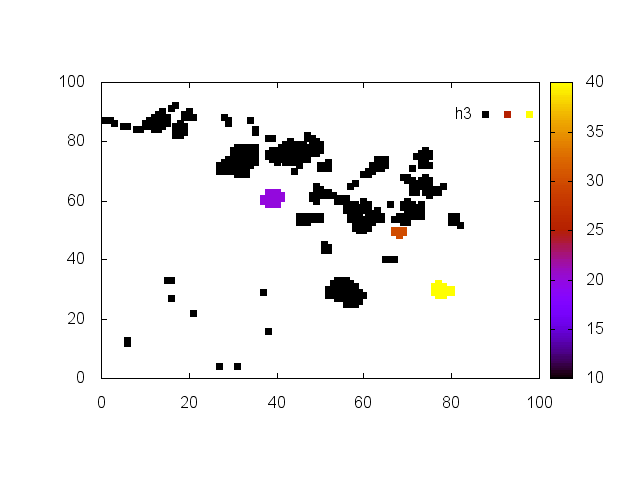
\includegraphics[scale=.3]{./img/stampe/scc1/3.png}
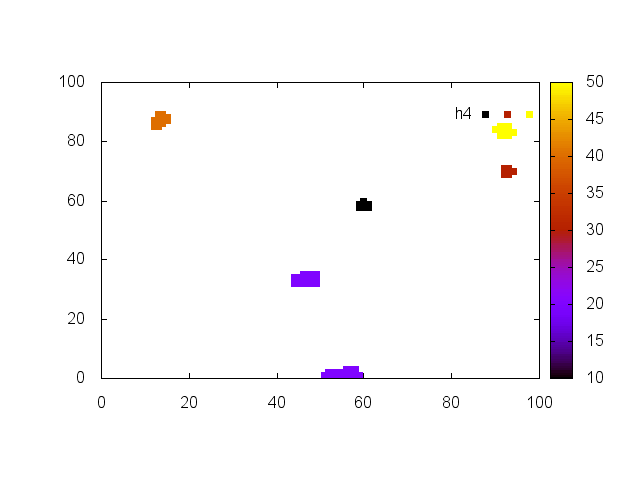
\includegraphics[scale=.3]{./img/stampe/scc1/4.png}
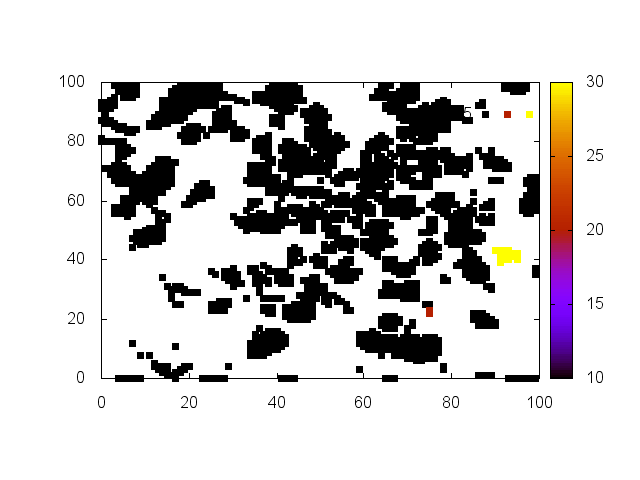
\includegraphics[scale=.3]{./img/stampe/scc1/5.png}
\end{subfigure}

\begin{subfigure}[b]{1\textwidth}
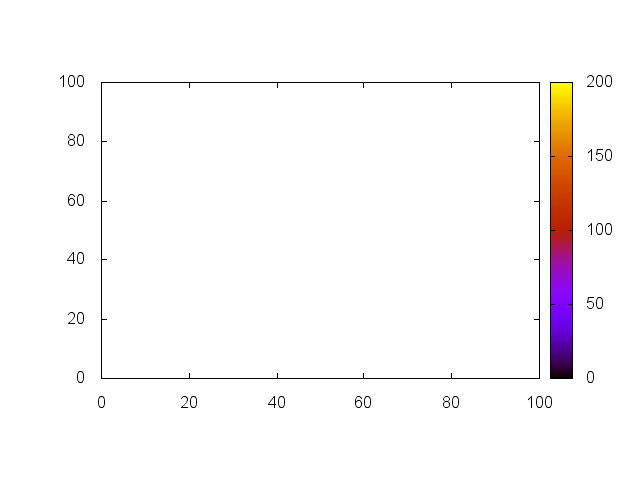
\includegraphics[scale=.3]{./img/stampe/scc1/6.png}
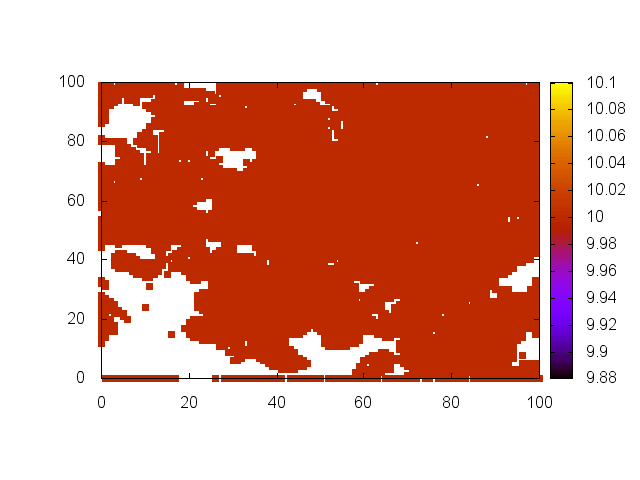
\includegraphics[scale=.3]{./img/stampe/scc1/7.png}
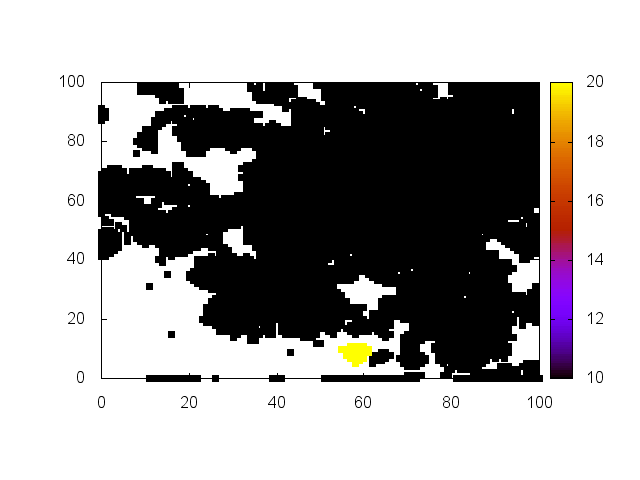
\includegraphics[scale=.3]{./img/stampe/scc1/8.png}
\end{subfigure}
\begin{subfigure}[b]{1\textwidth}
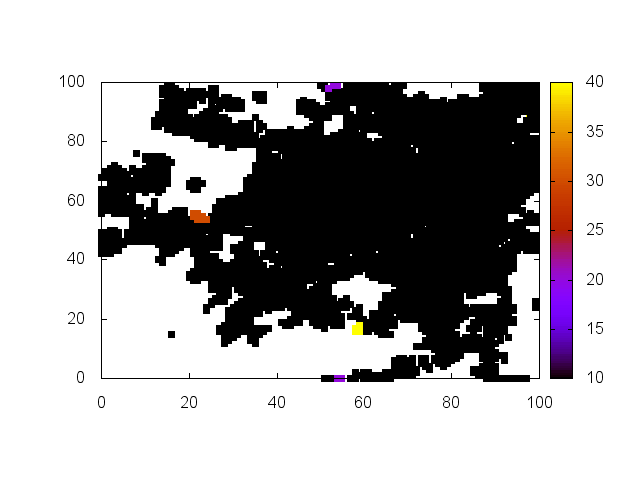
\includegraphics[scale=.3]{./img/stampe/scc1/9.png}
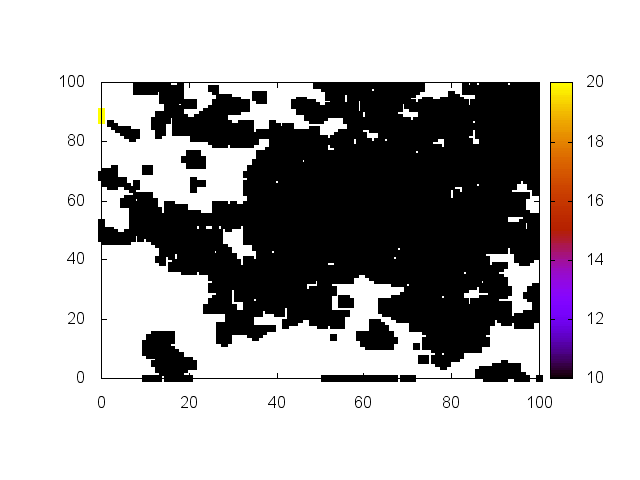
\includegraphics[scale=.3]{./img/stampe/scc1/10.png}
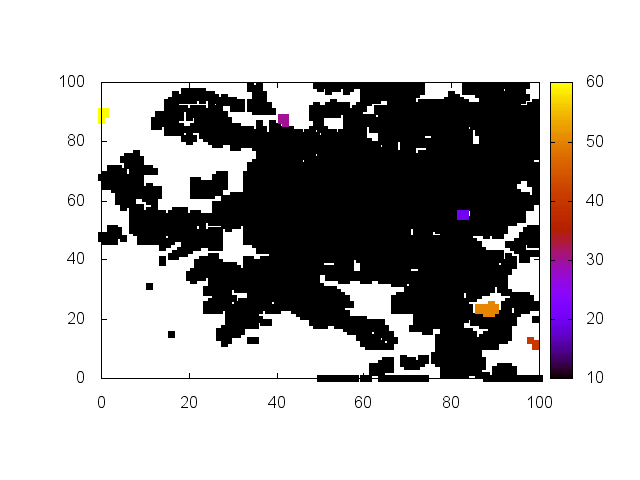
\includegraphics[scale=.3]{./img/stampe/scc1/11.png}
\end{subfigure}
\caption{SCC1, Taglio 0.005, h 0-11. Da vedere da sinistra verso destra e dall'alto verso il basso}
\end{figure}
\begin{figure}
\begin{subfigure}[b]{1\textwidth}
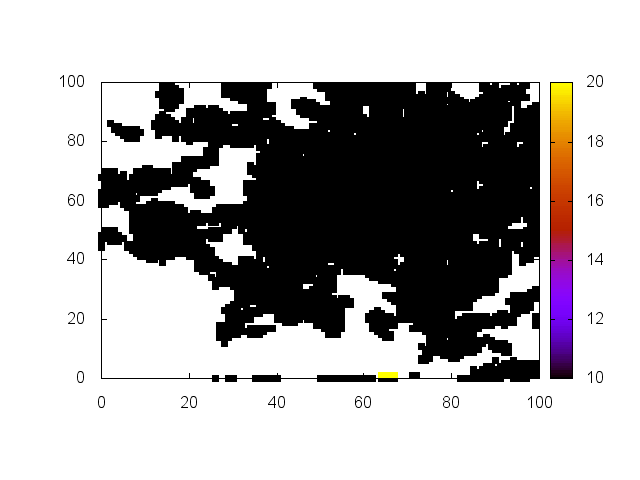
\includegraphics[scale=.3]{./img/stampe/scc1/12.png}
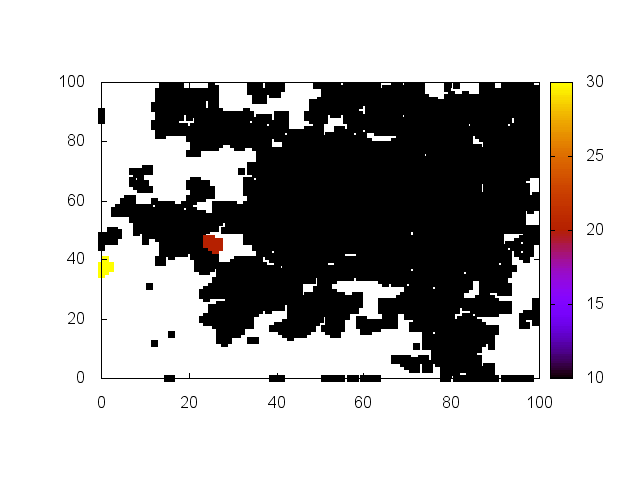
\includegraphics[scale=.3]{./img/stampe/scc1/13.png}
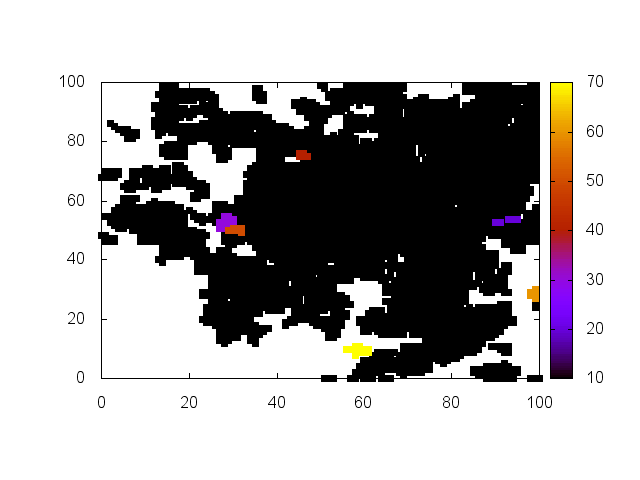
\includegraphics[scale=.3]{./img/stampe/scc1/14.png}
\end{subfigure}
\begin{subfigure}[b]{1\textwidth}
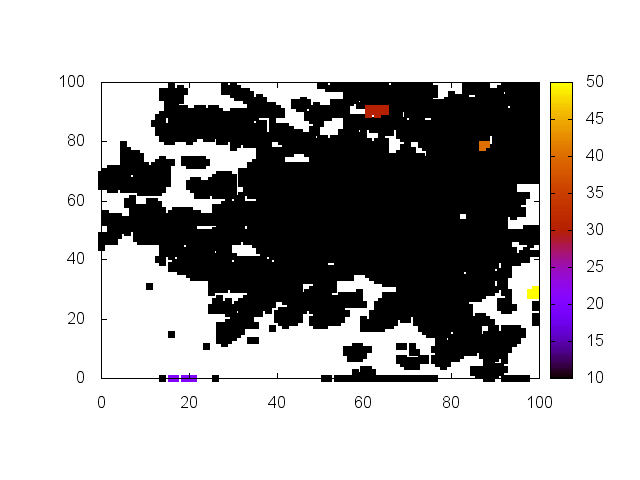
\includegraphics[scale=.3]{./img/stampe/scc1/15.png}
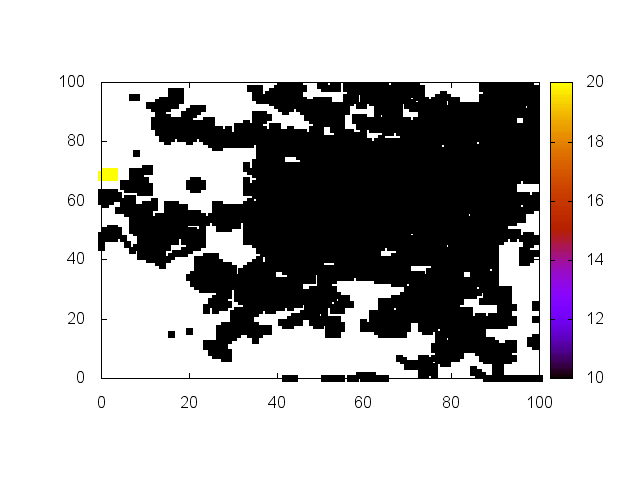
\includegraphics[scale=.3]{./img/stampe/scc1/16.png}
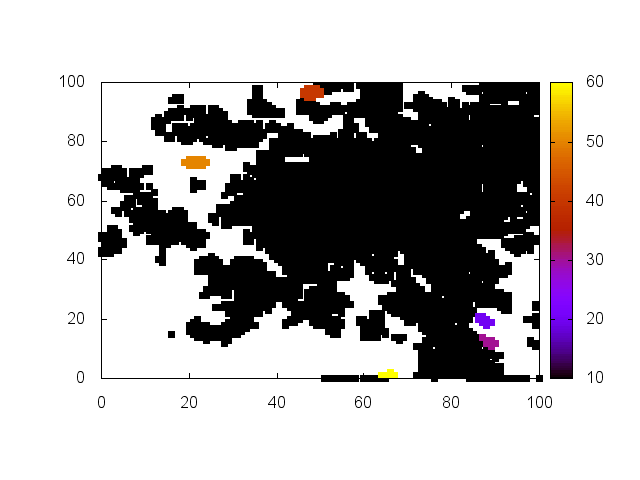
\includegraphics[scale=.3]{./img/stampe/scc1/17.png}
\end{subfigure}
\begin{subfigure}[b]{1\textwidth}
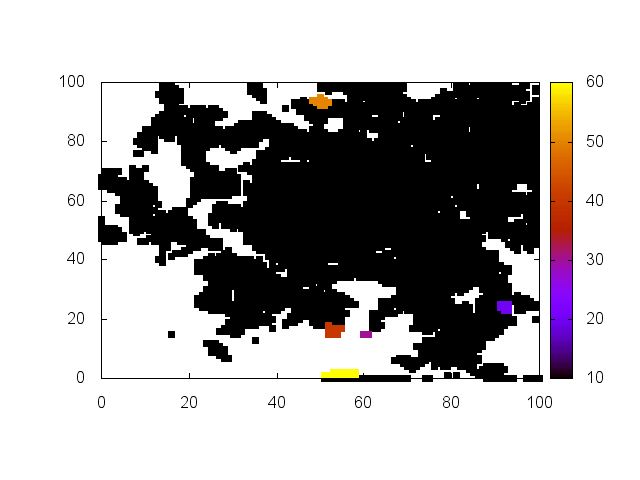
\includegraphics[scale=.3]{./img/stampe/scc1/18.png}
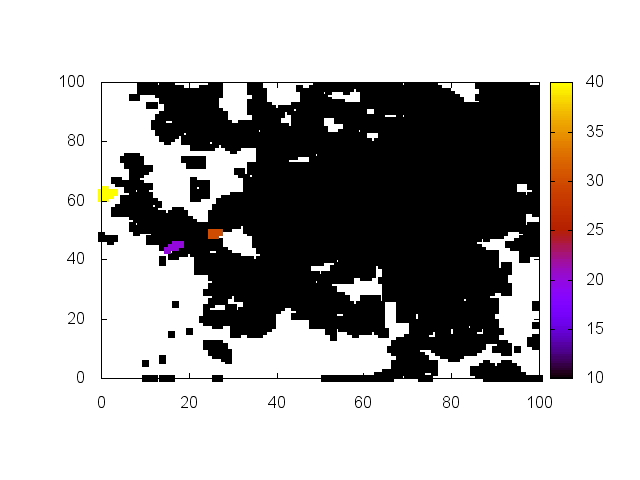
\includegraphics[scale=.3]{./img/stampe/scc1/19.png}
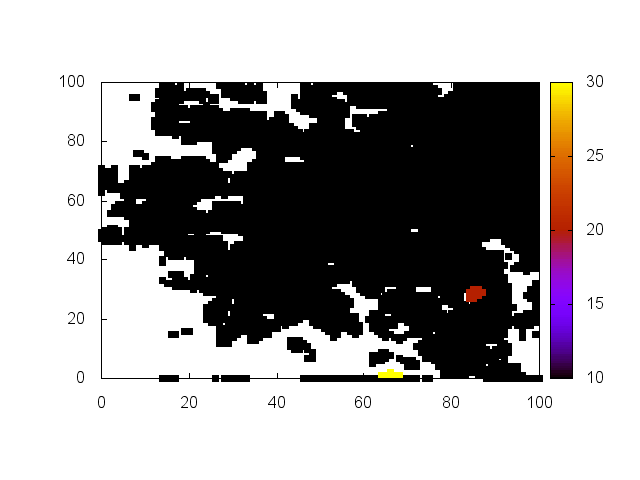
\includegraphics[scale=.3]{./img/stampe/scc1/20.png}
\end{subfigure}
\begin{subfigure}[b]{1\textwidth}
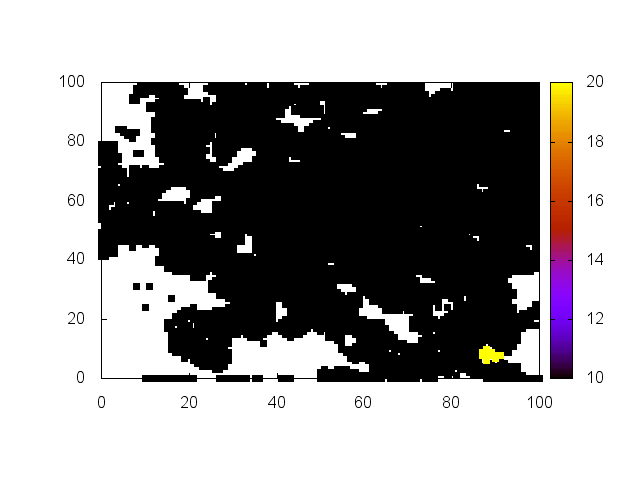
\includegraphics[scale=.3]{./img/stampe/scc1/21.png}
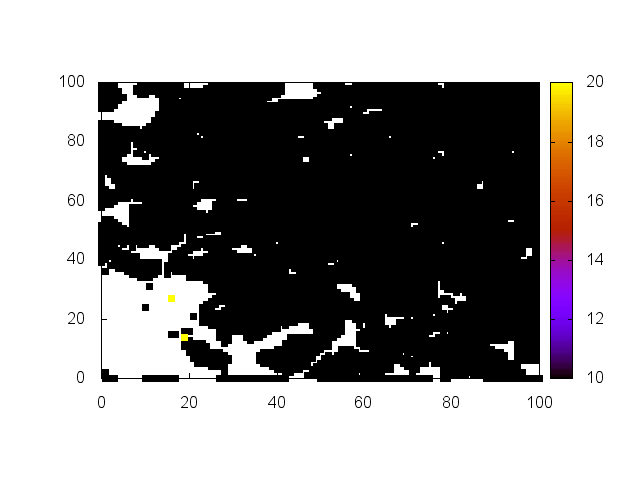
\includegraphics[scale=.3]{./img/stampe/scc1/22.png}
\end{subfigure}
\caption{SCC1, Taglio 0.005, h 12-22; da vedersi da sinistra verso destra e dell'alto verso il basso.}
\end{figure}

Come esempio per tutti i casi SCC riportiamo il caso SCC 1 con taglio degli archi con valore minore di
0.005. In questo caso, le componenti sono per la maggior parte delle ore estremamente ampie, come si può vedere in seguito:
\begin{figure}
\begin{verbatim}
0:      6,
1:      2972,11,
2:      4,2,13,10,38,40,9,
3:      462,19,7,16,
4:      7,41,7,14,14,
5:      2563,2,18,
6:
7:      8010,
8:      6605,29,
9:      5677,5,8,5,
10:     5638,4,
11:     5492,4,5,3,13,6,
12:     5729,4,
13:     5692,14,11,
14:     5818,5,13,5,8,6,12,
15:     5784,5,12,3,5,
16:     5362,11,
17:     5118,9,7,15,14,5,
18:     5623,8,2,11,11,14,
19:     5951,5,5,10,
20:     6676,11,6,
21:     7449,12,
22:     7971,2,
\end{verbatim}
\caption{Nel listato, per ogni ora (alla sinistra), una lista delle dimensioni delle CFC trovate}
\label{list:scc1_0-005}
\end{figure}

Si noti in ~\ref{list:scc1_0-005} come la dimensione delle componenti può variare anche notevolmente a seconda del traffico presente in un'ora. Questo potrebbe essere dovuto al fatto che il taglio è estremamente basso, e pertanto agisce solamente su una parte minima degli archi. Nelle ore in cui il traffico è minore, anche le componenti hanno dimensioni notevolmente minori: probabilmente questo è dovuto al fatto che il numero di archi uscenti (fuori dall'orario lavorativo) è minore e con probabilità maggiore.


%\subsection{SCC1, taglio 0.05}
%In questo caso, invece, le dimensioni delle componenti fortemente connesse diminuiscono notevolmente. Si noti, a conferma dell'ipotesi fatta in \ref{scc1_0-005}, come le dimensioni delle CFC calino drasticamente nelle ore di maggior traffico, mentre le ore che hanno un traffico inferiore sono caratterizzate da CFC più ampie.
%Si veda \ref{list:scc1_0-05}. Questo sembra indicare la necessità di effettuare tagli diversi per ore diverse, in modo da poter gestire diverse distribuzioni di traffico.
%\begin{figure}
%\begin{verbatim}
%0:      4,7,2,2,6,
%1:      383,2,4,7,7,6,6,9,5,9,2,
%2:      6,4,6,11,5,4,4,2,8,8,
%3:      5,6,5,11,9,
%4:      6,4,8,6,6,
%5:      8,4,3,5,8,3,7,2,3,
%6:      718,4,2,10,9,3,6,3,7,3,6,7,3,
%7:      115,6,2,2,3,2,2,2,3,4,
%8:      2,3,
%9:
%10:     2,2,
%11:     2,
%12:     3,
%13:     2,
%14:
%15:     4,
%16:
%17:     2,
%18:     4,5,5,
%19:
%20:
%21:     2,2,2,2,4,5,2,5,
%22:     248,2,2,2,2,4,2,6,6,4,2,2,2,2,9,
%\end{verbatim}
%\caption{Da leggersi come in \ref{list:scc1_0-005}}
%\label{list:scc1_0-05}
%\end{figure}
%Il risultato ottenuto, anche in questo caso non è stato considerato soddisfacente. Come esempio, mostriamo in \ref{list:scc1_0-05_1011cfc} le componenti fortemente connesse trovate alle ore 10 e alle ore 11. Oltre alla loro dimensione - certamente non eccessiva - si può vedere che le CFC in 10 scompaiono in 11.
%Il dato confortante è che le CFC sono contigue geograficamente; ciò parebbe confermare l'ipotesi di una correlazione tra frequenza delle chiamate e vicinanza geografica.
%\begin{figure}
%\begin{subfigure}[b]{1\textwidth}
%\begin{verbatim}
%==== 10.cfc
%{7249,7250}
%{7724,7824}
%\end{verbatim}
%\begin{verbatim}
%====11.cfc
%{3659,3660}
%\end{verbatim}
%\end{subfigure}
%\caption{Le CFC trovate alle ore 10 e alle ore 11 del 15 Novembre 2013}
%\label{list:scc1_0-05_1011cfc}
%\end{figure}
%\subsection{SCC2, taglio 0.005}
%Il comportamento evidenziato con questo tipo di visita, che, ricordiamo, seleziona prima i nodi con minore traffico e dalla stella uscenti quelli con minore probabilità, non danno risultati estremamente diversi.
%%todo: continuare.

\subsubsection{Stable, taglio al 99-esimo percentile}


\begin{figure}
\centering

\begin{subfigure}[b]{1\textwidth}
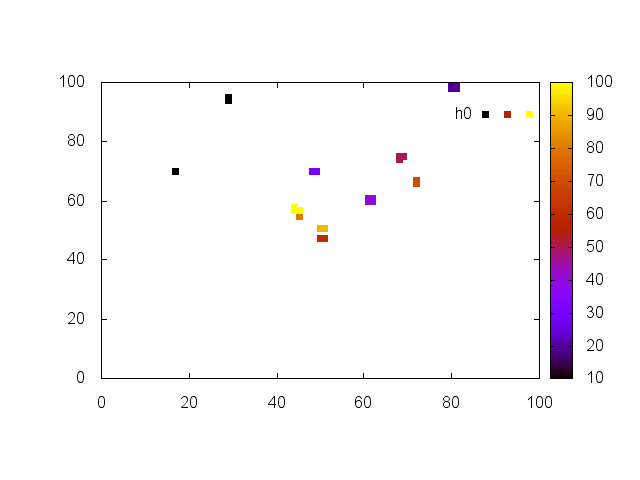
\includegraphics[scale=.3]{./img/SCC_Stable3/cut99p/0.png}
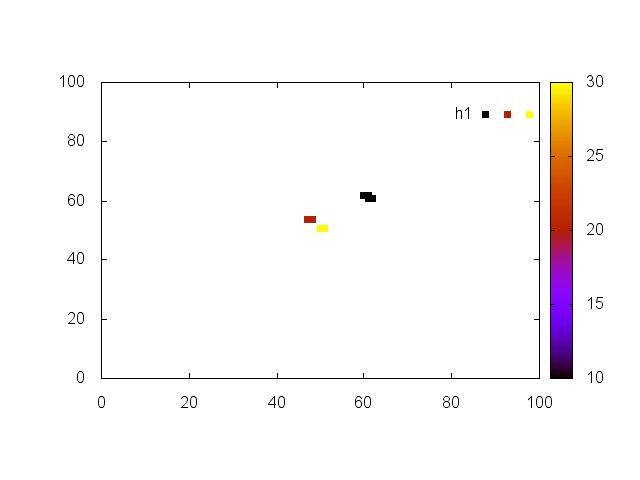
\includegraphics[scale=.3]{./img/SCC_Stable3/cut99p/1.png}
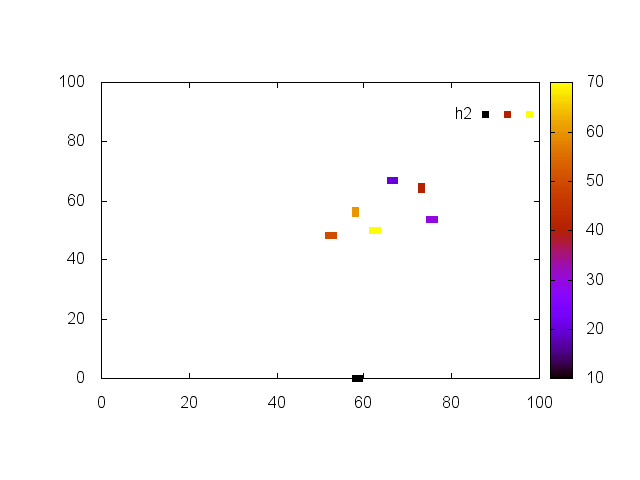
\includegraphics[scale=.3]{./img/SCC_Stable3/cut99p/2.png}
\end{subfigure}

\begin{subfigure}[b]{1\textwidth}
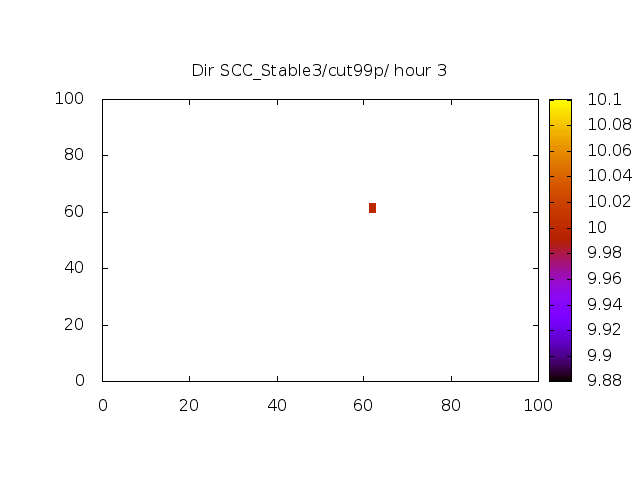
\includegraphics[scale=.3]{./img/SCC_Stable3/cut99p/3.png}
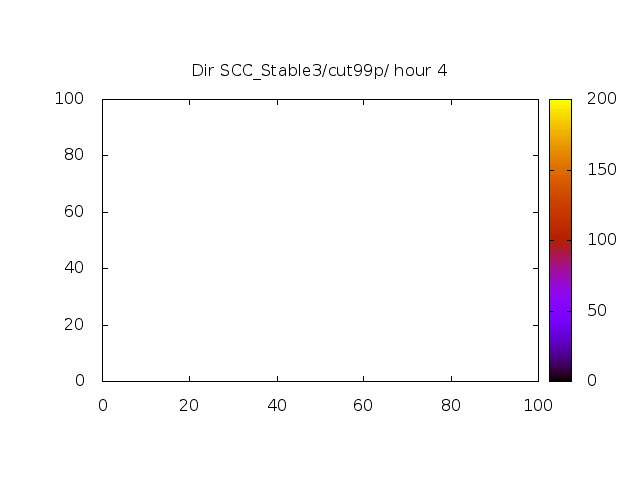
\includegraphics[scale=.3]{./img/SCC_Stable3/cut99p/4.png}
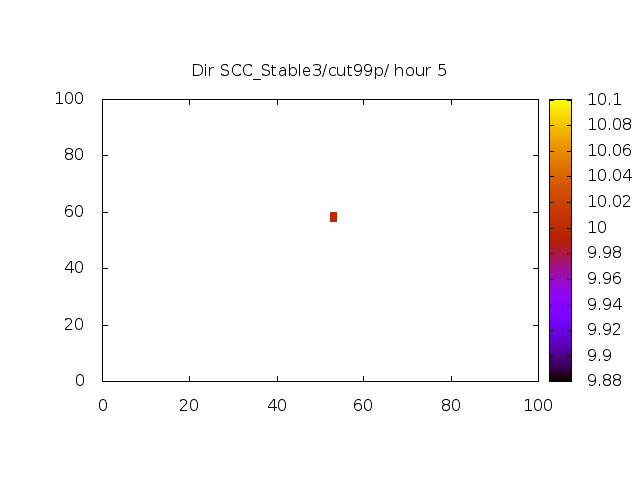
\includegraphics[scale=.3]{./img/SCC_Stable3/cut99p/5.png}
\end{subfigure}

\begin{subfigure}[b]{1\textwidth}
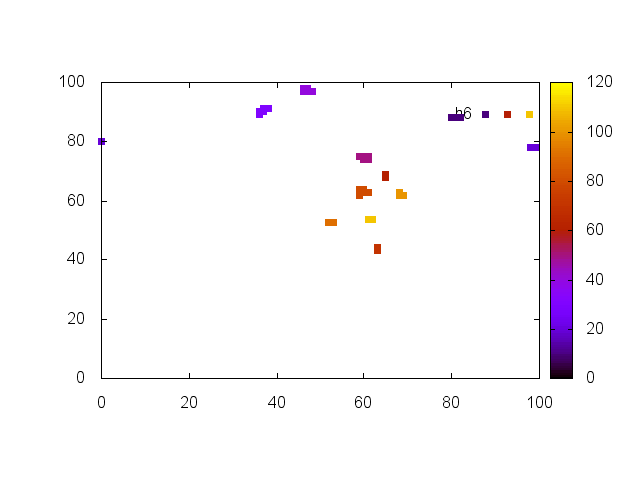
\includegraphics[scale=.3]{./img/SCC_Stable3/cut99p/6.png}
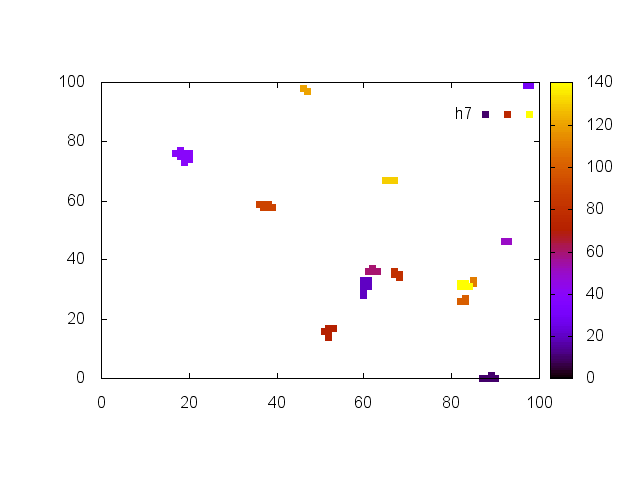
\includegraphics[scale=.3]{./img/SCC_Stable3/cut99p/7.png}
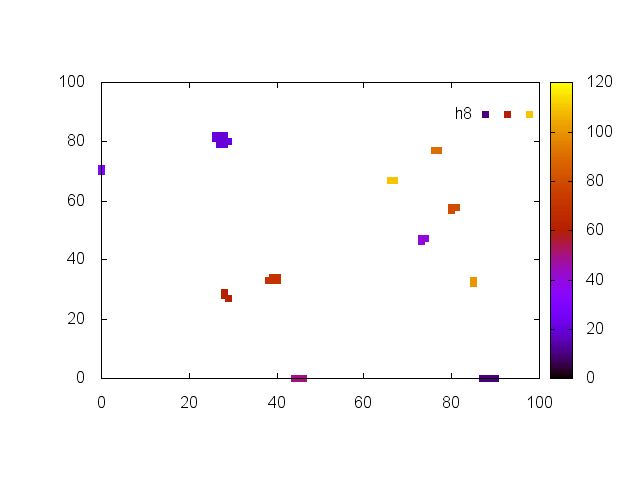
\includegraphics[scale=.3]{./img/SCC_Stable3/cut99p/8.png}
\end{subfigure}
\begin{subfigure}[b]{1\textwidth}
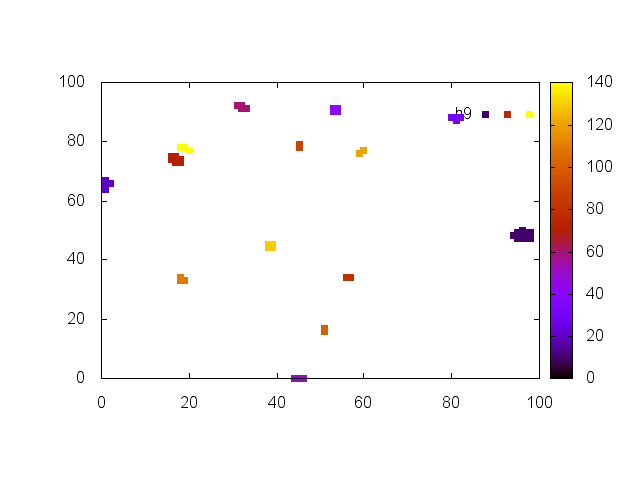
\includegraphics[scale=.3]{./img/SCC_Stable3/cut99p/9.png}
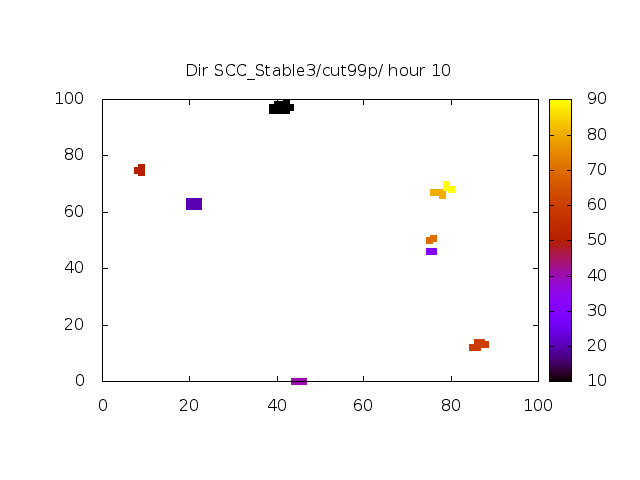
\includegraphics[scale=.3]{./img/SCC_Stable3/cut99p/10.png}
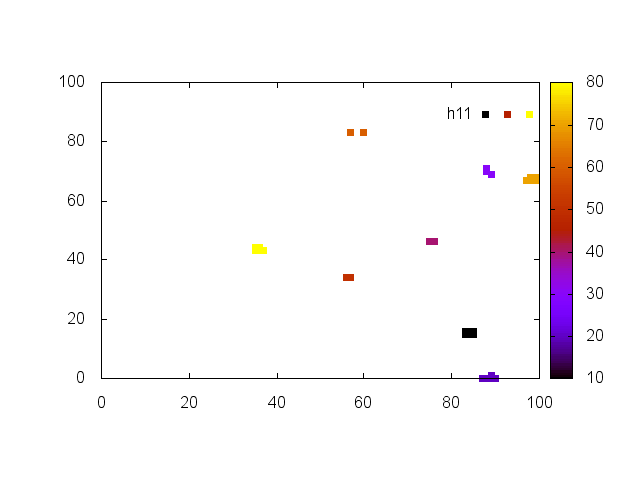
\includegraphics[scale=.3]{./img/SCC_Stable3/cut99p/11.png}
\end{subfigure}
\caption{Stable, Taglio 99-esimo percentile, h 0-11. Da vedere da sinistra verso destra e dall'alto verso il basso}
\end{figure}


\begin{figure}
\centering

\begin{subfigure}[b]{1\textwidth}
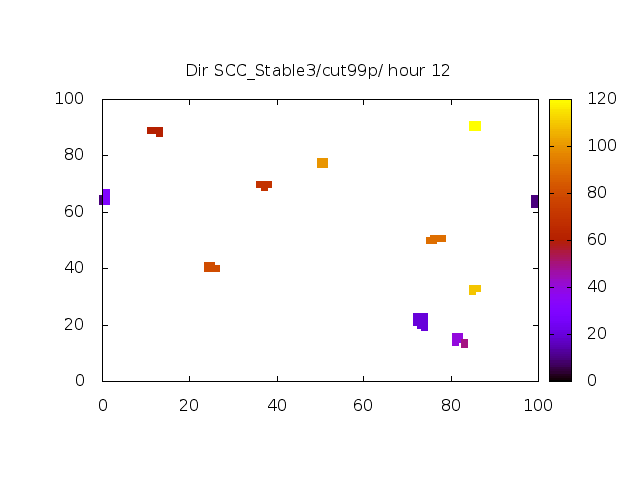
\includegraphics[scale=.3]{./img/SCC_Stable3/cut99p/12.png}
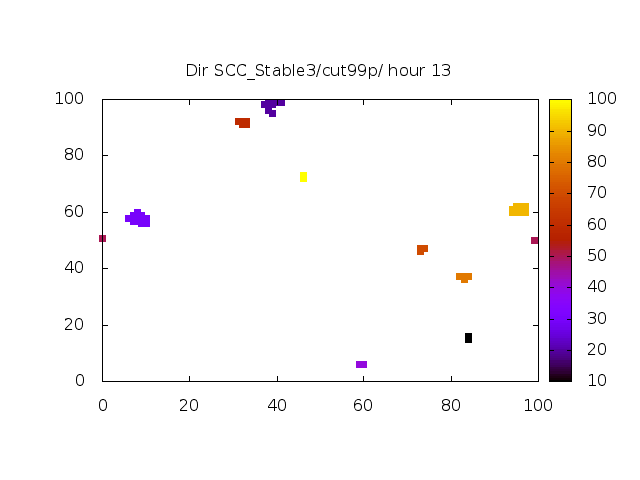
\includegraphics[scale=.3]{./img/SCC_Stable3/cut99p/13.png}
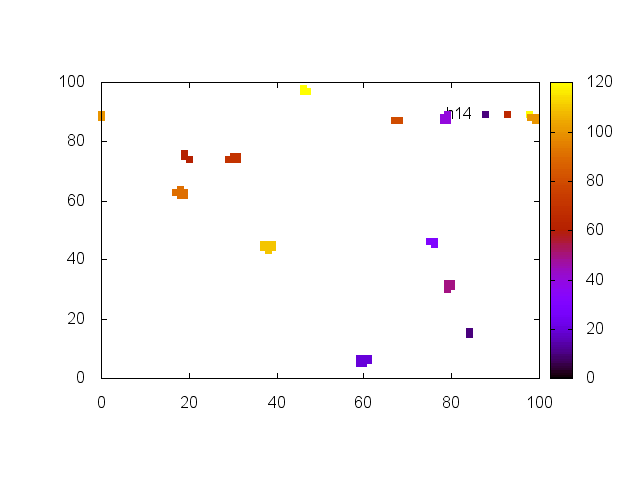
\includegraphics[scale=.3]{./img/SCC_Stable3/cut99p/14.png}
\end{subfigure}

\begin{subfigure}[b]{1\textwidth}
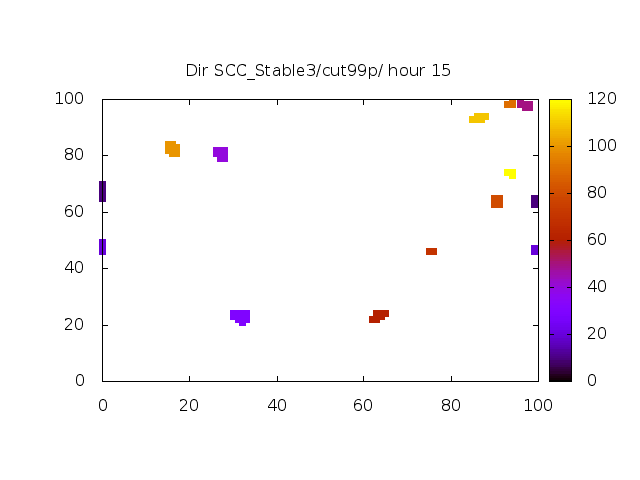
\includegraphics[scale=.3]{./img/SCC_Stable3/cut99p/15.png}
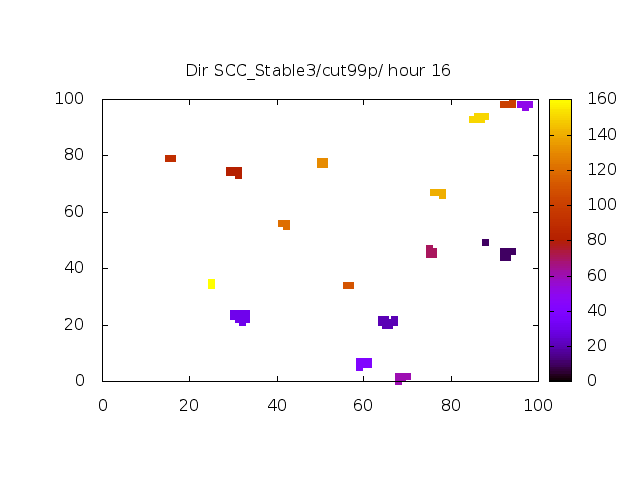
\includegraphics[scale=.3]{./img/SCC_Stable3/cut99p/16.png}
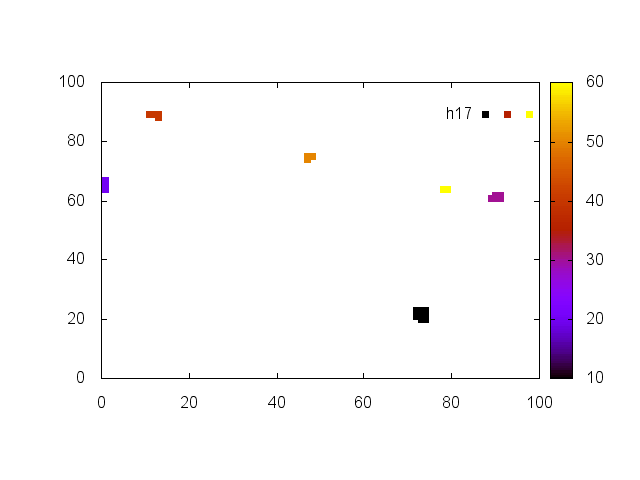
\includegraphics[scale=.3]{./img/SCC_Stable3/cut99p/17.png}
\end{subfigure}

\begin{subfigure}[b]{1\textwidth}
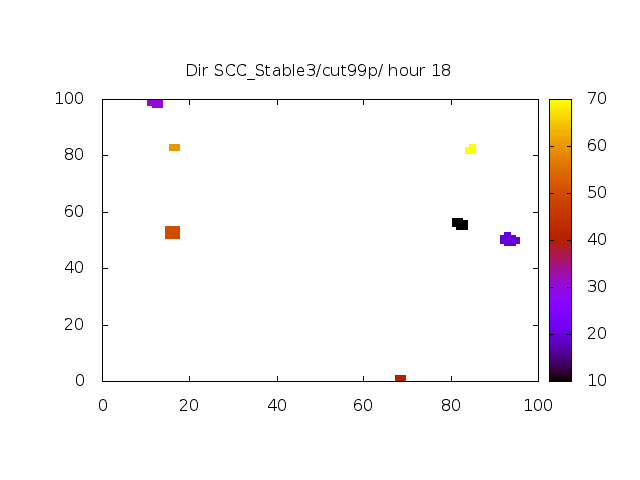
\includegraphics[scale=.3]{./img/SCC_Stable3/cut99p/18.png}
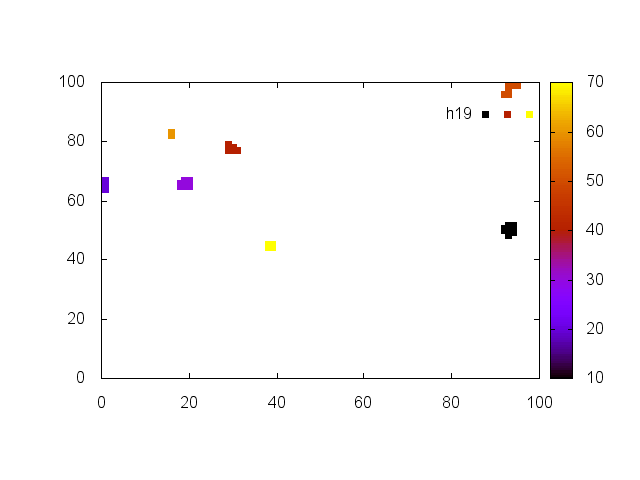
\includegraphics[scale=.3]{./img/SCC_Stable3/cut99p/19.png}
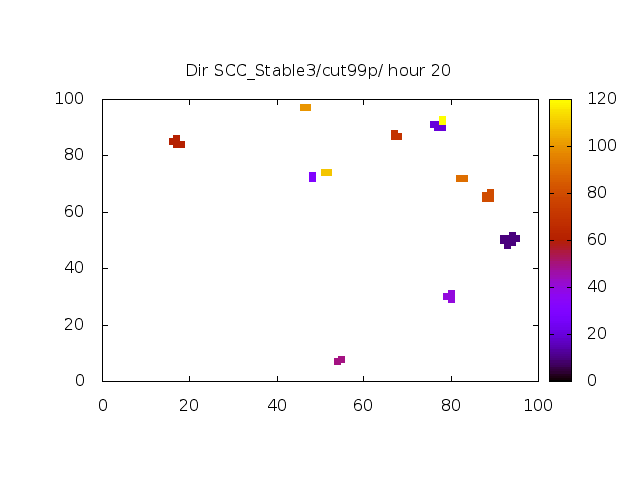
\includegraphics[scale=.3]{./img/SCC_Stable3/cut99p/20.png}
\end{subfigure}
\begin{subfigure}[b]{1\textwidth}
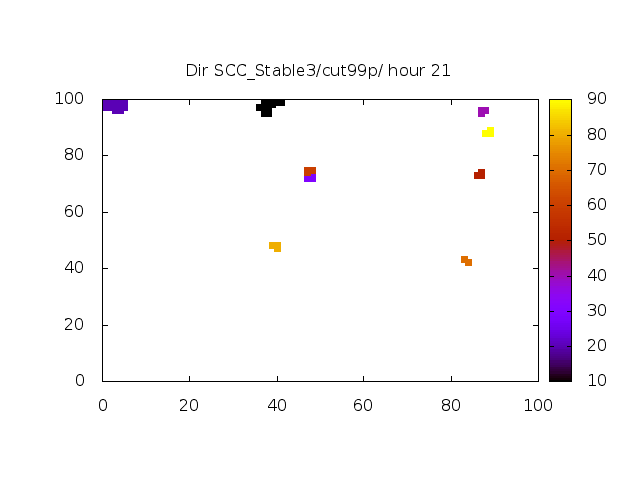
\includegraphics[scale=.3]{./img/SCC_Stable3/cut99p/21.png}
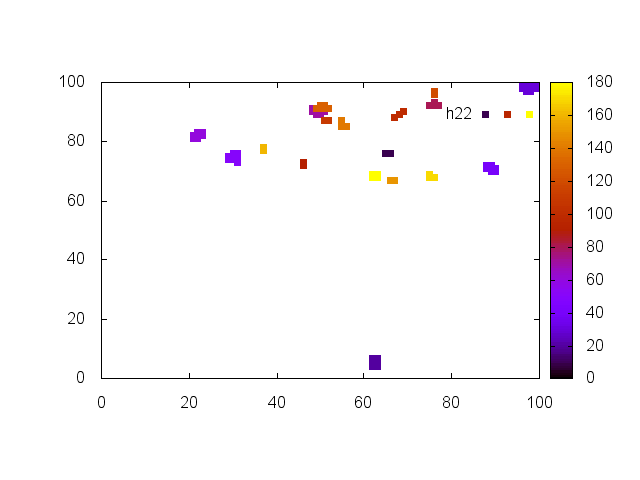
\includegraphics[scale=.3]{./img/SCC_Stable3/cut99p/22.png}
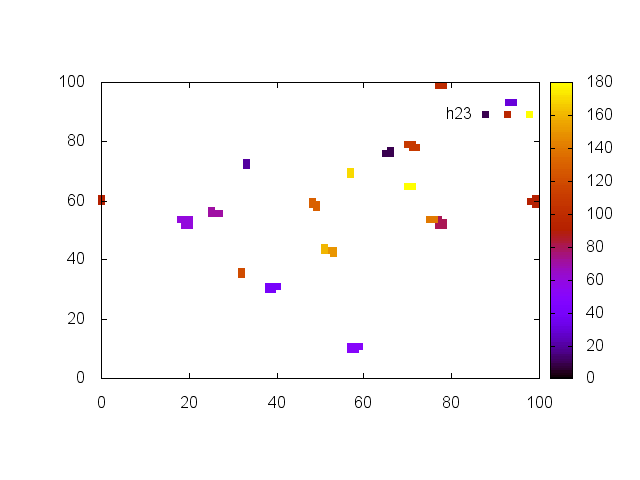
\includegraphics[scale=.3]{./img/SCC_Stable3/cut99p/23.png}
\end{subfigure}
\caption{Stable, Taglio 99-esimo percentile, h 12-23. Da vedere da sinistra verso destra e dall'alto verso il basso}
\end{figure}


\subsubsection{Stable, taglio al 95-esimo percentile}

\begin{figure}
\centering
\begin{subfigure}[b]{1\textwidth}
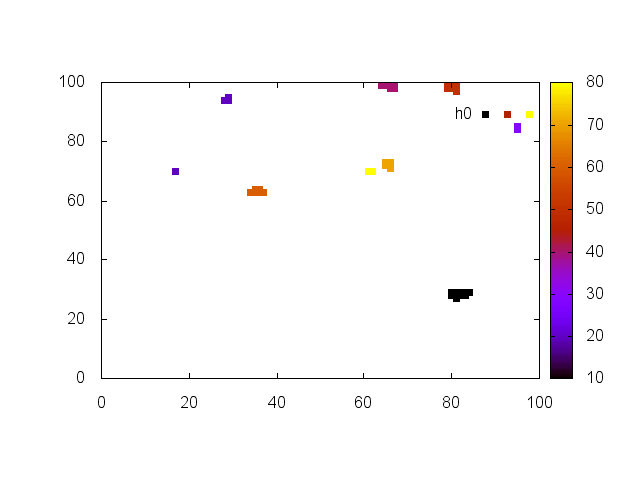
\includegraphics[scale=.3]{./img/SCC_Stable3/cut95p/0.png}
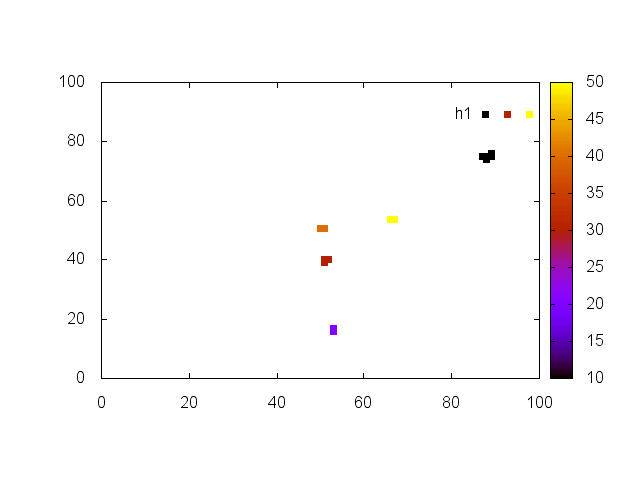
\includegraphics[scale=.3]{./img/SCC_Stable3/cut95p/1.png}
\includegraphics[scale=.3]{./img/SCC_Stable3/cut95p/2.png}
\end{subfigure}

\begin{subfigure}[b]{1\textwidth}
\includegraphics[scale=.3]{./img/SCC_Stable3/cut95p/3.png}
\includegraphics[scale=.3]{./img/SCC_Stable3/cut95p/4.png}
\includegraphics[scale=.3]{./img/SCC_Stable3/cut95p/5.png}
\end{subfigure}

\begin{subfigure}[b]{1\textwidth}
\includegraphics[scale=.3]{./img/SCC_Stable3/cut95p/6.png}
\includegraphics[scale=.3]{./img/SCC_Stable3/cut95p/7.png}
\includegraphics[scale=.3]{./img/SCC_Stable3/cut95p/8.png}
\end{subfigure}
\begin{subfigure}[b]{1\textwidth}
\includegraphics[scale=.3]{./img/SCC_Stable3/cut95p/9.png}
\includegraphics[scale=.3]{./img/SCC_Stable3/cut95p/10.png}
\includegraphics[scale=.3]{./img/SCC_Stable3/cut95p/11.png}
\end{subfigure}
\caption{Stable, Taglio 95-esimo percentile, h 0-11. Da vedere da sinistra verso destra e dall'alto verso il basso}
\end{figure}

\begin{figure}
\centering

\begin{subfigure}[b]{1\textwidth}
\includegraphics[scale=.3]{./img/SCC_Stable3/cut95p/12.png}
\includegraphics[scale=.3]{./img/SCC_Stable3/cut95p/13.png}
\includegraphics[scale=.3]{./img/SCC_Stable3/cut95p/14.png}
\end{subfigure}

\begin{subfigure}[b]{1\textwidth}
\includegraphics[scale=.3]{./img/SCC_Stable3/cut95p/15.png}
\includegraphics[scale=.3]{./img/SCC_Stable3/cut95p/16.png}
\includegraphics[scale=.3]{./img/SCC_Stable3/cut95p/17.png}
\end{subfigure}

\begin{subfigure}[b]{1\textwidth}
\includegraphics[scale=.3]{./img/SCC_Stable3/cut95p/18.png}
\includegraphics[scale=.3]{./img/SCC_Stable3/cut95p/19.png}
\includegraphics[scale=.3]{./img/SCC_Stable3/cut95p/20.png}
\end{subfigure}
\begin{subfigure}[b]{1\textwidth}
\includegraphics[scale=.3]{./img/SCC_Stable3/cut95p/21.png}
\includegraphics[scale=.3]{./img/SCC_Stable3/cut95p/22.png}
\includegraphics[scale=.3]{./img/SCC_Stable3/cut95p/23.png}
\end{subfigure}
\caption{Stable, Taglio 95-esimo percentile, h 12-23. Da vedere da sinistra verso destra e dall'alto verso il basso}
\end{figure}

\subsubsection{Stable, taglio al 90-esimo percentile}

\begin{figure}
\centering
\begin{subfigure}[b]{1\textwidth}
\includegraphics[scale=.3]{./img/SCC_Stable3/cut90p/0.png}
\includegraphics[scale=.3]{./img/SCC_Stable3/cut90p/1.png}
\includegraphics[scale=.3]{./img/SCC_Stable3/cut90p/2.png}
\end{subfigure}

\begin{subfigure}[b]{1\textwidth}
\includegraphics[scale=.3]{./img/SCC_Stable3/cut90p/3.png}
\includegraphics[scale=.3]{./img/SCC_Stable3/cut90p/4.png}
\includegraphics[scale=.3]{./img/SCC_Stable3/cut90p/5.png}
\end{subfigure}

\begin{subfigure}[b]{1\textwidth}
\includegraphics[scale=.3]{./img/SCC_Stable3/cut90p/6.png}
\includegraphics[scale=.3]{./img/SCC_Stable3/cut90p/7.png}
\includegraphics[scale=.3]{./img/SCC_Stable3/cut90p/8.png}
\end{subfigure}
\begin{subfigure}[b]{1\textwidth}
\includegraphics[scale=.3]{./img/SCC_Stable3/cut90p/9.png}
\includegraphics[scale=.3]{./img/SCC_Stable3/cut90p/10.png}
\includegraphics[scale=.3]{./img/SCC_Stable3/cut90p/11.png}
\end{subfigure}
\caption{Stable, Taglio 90-esimo percentile, h 0-11. Da vedere da sinistra verso destra e dall'alto verso il basso}
\end{figure}

\begin{figure}
\centering

\begin{subfigure}[b]{1\textwidth}
\includegraphics[scale=.3]{./img/SCC_Stable3/cut90p/12.png}
\includegraphics[scale=.3]{./img/SCC_Stable3/cut90p/13.png}
\includegraphics[scale=.3]{./img/SCC_Stable3/cut90p/14.png}
\end{subfigure}

\begin{subfigure}[b]{1\textwidth}
\includegraphics[scale=.3]{./img/SCC_Stable3/cut90p/15.png}
\includegraphics[scale=.3]{./img/SCC_Stable3/cut90p/16.png}
\includegraphics[scale=.3]{./img/SCC_Stable3/cut90p/17.png}
\end{subfigure}

\begin{subfigure}[b]{1\textwidth}
\includegraphics[scale=.3]{./img/SCC_Stable3/cut90p/18.png}
\includegraphics[scale=.3]{./img/SCC_Stable3/cut90p/19.png}
\includegraphics[scale=.3]{./img/SCC_Stable3/cut90p/20.png}
\end{subfigure}
\begin{subfigure}[b]{1\textwidth}
\includegraphics[scale=.3]{./img/SCC_Stable3/cut90p/21.png}
\includegraphics[scale=.3]{./img/SCC_Stable3/cut90p/22.png}
\includegraphics[scale=.3]{./img/SCC_Stable3/cut90p/23.png}
\end{subfigure}
\caption{Stable, Taglio 90-esimo percentile, h 12-23. Da vedere da sinistra verso destra e dall'alto verso il basso}
\end{figure}

\section{Alcune conclusioni}

\begin{enumerate}
\item Occorre effettuare tagli con valore molto alto perchè il grafo è inerentemente fortemente connesso.
\item Le statistiche sulle probabilità degli archi denotano l'effettiva esistenza di square che si chiamano
più degli altri negli orari non lavorativi.
\item La strategia di visita incide molto nella formazione del risultato e probabilmente il problema di
non considerare mai due volte lo stesso nodo può eliminare delle CFC interessanti.
\item Il numero di CFC è più basso di quello attesa, tuttavia le CFC sono ben distribuite spazialmente 
sulla grid; si noti anche come al variare delle fasce orarie variano le zone in cui vengono scoperte
le CFC.
\item Sopratutto nelle ore di minor traffico si individuano principalmente CFC che potrebbero essere
fatte risalire alla presenza di paesi della periferia di Milano (la grid copre un'area molto più grande
della sola zona urbana di Milano).
\item Le CFC trovate non mostrano persistenza (salvo rare eccezioni) in fasce orarie contigue ma tendono
ad apparire e scomparire. Si noti come questo non può essere dovuto al valore del taglio, perchè
i percentili vengono calcolati per ogni fascia oraria.
\end{enumerate}

\section{Prosecuzione del lavoro}

\begin{enumerate}
\item Implementazione di tutta l'analisi su Hadoop.
\item Cercare le  componenti debolmente connesse.
\item Strategie di clustering.
\item Ampliare il periodo analizzato per includere tutti i giorni di novembre e dicembre (da decidere
come aggregare i risultati giornalieri)
\item affinare il periodo di aggregazione? (e.g. passare a fasce di 30 min)
\end{enumerate}

\end{document}
